%Imports
\usepackage{graphicx,abstract,epstopdf,times,authblk,geometry,fancyhdr,etoolbox,caption,sectsty,float, amsmath}
\usepackage[sort,round]{natbib}

%Margins
\newgeometry{top=2cm,left=2.5cm,right=2.5cm,bottom=4.5cm}

%Header
\addtolength{\headheight}{1.5cm}
\pagestyle{fancyplain}
\lhead{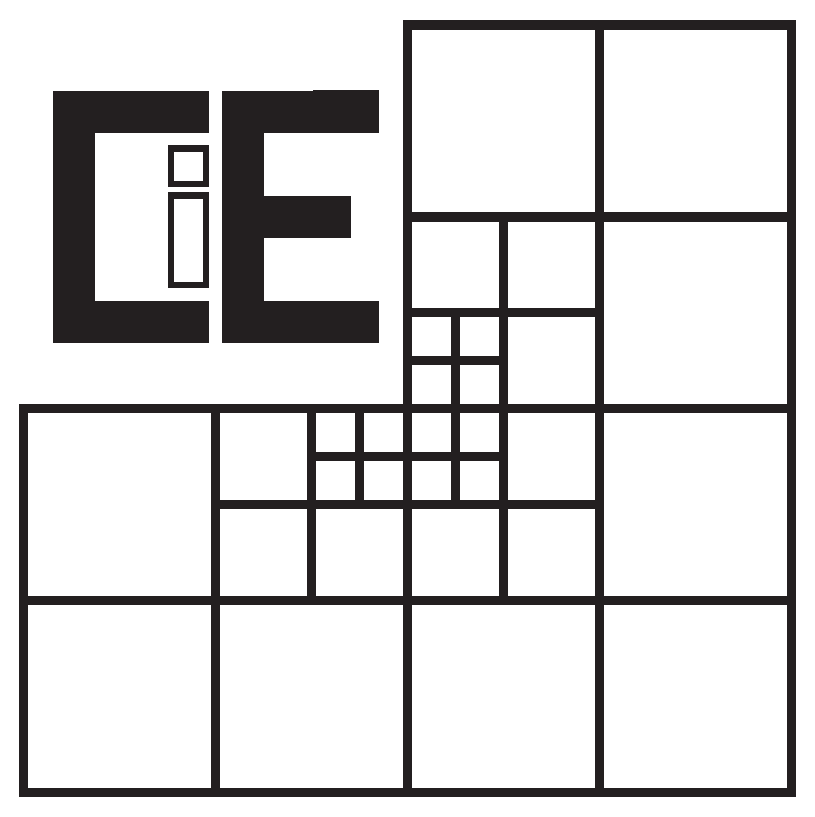
\includegraphics[height=1.3cm]{src/logo.eps} Chair of Computation in Engineering}
\rhead{Software-Lab 2015}
\renewcommand{\headrulewidth}{0pt}

%Layout
\renewcommand\Authfont{\fontsize{10pt}{9pt}\selectfont }
\renewcommand\Affilfont{\fontsize{10pt}{9pt}\selectfont }
\renewcommand\Authands{, }
\renewcommand{\abstractname}{\vspace{-\baselineskip}}
\renewcommand{\abstracttextfont}{\fontsize{10pt}{12pt}\selectfont\noindent\textbf{Abstract. }}
\date{\vspace{-\baselineskip}\vspace{-\baselineskip}}
\captionsetup{font=small}
\allsectionsfont{\fontsize{12pt}{14pt}\selectfont\bfseries }
\renewcommand{\arraystretch}{1.8}
\AtBeginEnvironment{tabular}{\fontsize{10pt}{9pt}\selectfont}
\bibliographystyle{src/agsm}
\newcommand\emails{\affil[ ]}

\usepackage[colorinlistoftodos]{todonotes}

% For our todos we use the following colorcode:
% intern: only internal info, dont care
% urgent: all please have a look at it
% done: task solved, but would not mind a second person having a look at it

% the following todo commands take the arguments 
% \todo...[options]{author}{todomessage}
% options are the common options from the todonotes package and are an optional parameter
% for \todoin...[options]{author}{todomessage}{section}
% where todoin marks a whole section for refactoring or similar. 
\newcommand{\tododone}[3][noinline]{\todo[#1, author = #2, color=green!40]{\textit{#3}}}
\newcommand{\todointern}[3][noinline]{\todo[#1, author = #2, color=blue!40]{#3}}
\newcommand{\todourgent}[3][noinline]{\todo[#1, author = #2, color=red!40]{\textbf{#3}}}
\newcommand\todoindone[4][]{\todo[inline, author = #2, caption={#3}, #1, color=green!40]{
\begin{minipage}{\textwidth-4pt}\underline{#3}\\ \textit{#4}\end{minipage}}}
\newcommand\todoinintern[4][]{\todo[inline, author = #2, caption={#3}, #1, color=blue!40]{
\begin{minipage}{\textwidth-4pt}\underline{#3}\\  #4\end{minipage}}}
\newcommand\todoinurgent[4][]{\todo[inline, author = #2, caption={#3}, #1, color=red!40]{
\begin{minipage}{\textwidth-4pt}\underline{#3}\\ \textbf{#4}\end{minipage}}}
